% Appendix C *** Appendix for chapter 5 now, labels remain "chapter 6" and "appendix C"

\chapter{Supplementary Data for Chapter 5}\label{AppendixC}
\lhead{Appendix B. \emph{Supplementary Data for Chapter 5}}

\section{The SIR Score}\label{appendixc/sir}

The SIR (Size of the Immune Repertoire) score \citep{Vider-Shalit2007} is a permutation measure where the number of predicted binders per allele is compared for each HTLV-I protein against a random protein of the same size. Briefly, for each protein-allele combination, the number of predicted strong binders ($< 50$ $nM$) and weak binders ($< 500$ $nM$) was found for both the consensus HTLV-I sequence and a randomized counterpart (using the amino acid frequencies present in HTLV-I). This ratio could then be used in place of the rank measure (\sref{RankMeasure}). There are a number of reasons though why this measure is not as effective as the rank measure for detecting the strength of binding to a given protein. Firstly, the SIR measure fails to take into account competition with other peptides for the same allele and secondly, it relates more to evolution i.e.~does this protein sequence contain more epitopes than would be expected? Therefore, one sequence could have a higher SIR score than another while containing fewer epitopes. However, it is useful to use as many independent methods as possible. Most of the tests outlined in \sref{chapter6Results} were repeated using the SIR measure (\tref{appendixc/table4}).The only finding that was not replicated was that the protective alleles A*0201 and Cw*08 bind HBZ more strongly than B*5401. We believe this is probably a question of power as we tested this hypothesis using a chi-squared table of the form:

\begin{table}[htp]
\begin{center}
\begin{tabular}{|c|c|c|}
\hline
 & \textbf{A*0201 \& Cw*0801} & \textbf{B5401} \bigstrut \\
\hline
\textbf{\# Predicted Epitopes} & A & B \bigstrut[t] \\
\textbf{\# Random Predicted Epitopes} & C & D \bigstrut[b] \\
\hline
\end{tabular}
\end{center}
\end{table}

But the numbers A-D were small (HBZ being poorly bound by most alleles, see \sref{chapter6/discussion}).

\begin{table}[htp]
\begin{center}

\begin{sideways}
{
\renewcommand{\arraystretch}{1.5}
\begin{tabulary}{1.5\textwidth}{|c|L|c|c|L|}
\hline
& Null hypothesis & SIR $< 50$ & SIR $< 500$ & Conclusion \\	
\hline
1 & Protective and detrimental alleles target HBZ equally & - & - & Not enough power for this test using the SIR measure \\
\hline
2 & AC and HAM/TSP patients target HBZ equally & 0.07 & 0.004 & ACs have HLA alleles that bind HBZ significantly more strongly compared to HAM/TSP patients \\
\hline
3 & There is no correlation between proviral load and the number of alleles that bind HBZ strongly & 0.014 & 0.01 & The higher the number of strong binding alleles to HBZ per individual, the lower their proviral load \\
\hline
4 & There is no correlation between load reduction (count) and disease prevalence reduction & 0.02 & 0.013 & Proteins that are strongly bound by asymptomatic carriers are, independently, those associated with a greater reduction in load when bound \\
\hline
\end{tabulary}
}
\end{sideways}
\end{center}

\caption[Binding analysis using the SIR measure]{The results of hypothesis testing using the SIR measure to define the strength of binding of HLA class I alleles to HBZ.}
\label{appendixc/table4}
\end{table}

%%%%%%%%%%%%%%%%%%%%%%%%%%%%%%%%%%%%%%%%%%%%%%%%%%%%%%%%%%%%%%%%%%%%%%%%%%%%%%%%%%%%%%%%%%%%%%%%%%%%
%%%%%%%%%%%%%%%%%%%%%%%%%%%%%%%%%%%%%%%%%%%%%%%%%%%%%%%%%%%%%%%%%%%%%%%%%%%%%%%%%%%%%%%%%%%%%%%%%%%%

\section{Multiple and logistic regression}\label{appendixc/log}

\cref{Chapter6}, \sref{chapter6/results/pred} described the power of peptide binding to predict proviral load, compared to associations with HLA genotype. For the analysis in \sref{chapter6/results/pred}, the binding strength of an individual's HLA class I repertoire to a specific HTLV-I protein was defined as the median rank value (see \sref{RankMeasure}) of the individual's A and B alleles. \tref{appendixc/tableMultRegress} compares this measure against other metrics defining the strength of binding of an individual's HLA class I alleles to a specific protein. Each model was tested on the HAM/TSP and AC groups separately. The HTLV-I proteins in the table are whose peptide - MHC class I binding ranks significantly explain a proportion (R$^2$) of the variance in proviral load. 5 different metrics were used. `Count' refers to the number of strong binding alleles that each individual posseses for a specific protein (\sref{RankMeasure}). `Median Rank' and `Median Affinity' refer to the median rank value or median raw predicted binding affinity of the individual's 4 A and B alleles (\sref{MethodsChapter6Result4}). Finally, `Max Rank' and `Max Affinity' refer to the highest rank value or median raw predicted binding affinity of the individual's 4 A and B alleles.

The targeting of HBZ is a significant predictor of proviral load in 5/10 of these models. In each case, the HBZ parameter coefficient is the `correct' sign for a beneficial effect of targeting HBZ: positive for the rank models where a low rank corresponds to strong binding and negative for the raw binding affinity scores where a high score corresponds to strong binding. 

We also tested some logistic regression models that predicted the disease status (asymptomatic or HAM/TSP) using predicted binding specificity to HTLV-I proteins as predictors. As in \tref{appendixc/tableMultRegress}, \tref{appendixc/tableLogRegress} shows the metric used for each model. As mentioned in \sref{Chapter6ResultFP}, these models are weakly predictive of disease status because of the many other determinants involved. However, they do illustrate again the effect of targeting HBZ, with 3/4 of the models showing HBZ as a significant beneficial predictor of HAM/TSP risk.

\begin{table}[htp]
\begin{center}
\begin{tabulary}{1.5\textwidth}{|c|c|c|c|c|c|}
\hline
Group & Method & $R^2$ & Protein & Effect & $P$ Value \bigstrut \\
\hline
AC & Count & 0.044029 & Env & 0.552145 & 0.002725 \bigstrut \\
\hline
\multirow{2}{*}{HAM} & \multirow{2}{*}{Count} & \multirow{2}{*}{0.059642} & Pol & 0.287735 & 0.044292 \bigstrut[t] \\
& & & Gag & -0.466769 & 0.000276 \bigstrut[b] \\
\hline
\multirow{2}{*}{AC} & \multirow{2}{*}{Median Rank} & \multirow{2}{*}{0.053639} & HBZ & 0.014960 & 0.000981 \bigstrut[t] \\
& & & Pro & -0.023219 & 0.012906 \bigstrut[b] \\
\hline
HAM & Median Rank & 0.025510 & HBZ & 0.003767 & 0.016983 \bigstrut \\
\hline
AC & Median Affinity & 0.025705 & HBZ & -1.216011 & 0.022650 \bigstrut \\
\hline
HAM & Median Affinity & 0.032798 & HBZ & -0.856337 & 0.006694 \bigstrut \\
\hline
\multirow{2}{*}{AC} & \multirow{2}{*}{Max Rank} & \multirow{2}{*}{0.048615} & Rof & -0.041019 & 0.025676 \bigstrut[t] \\
& & & P21 & 0.019808 & 0.016166 \bigstrut[b] \\
\hline
\multirow{3}{*}{HAM} & \multirow{3}{*}{Max Rank} & \multirow{3}{*}{0.082557} & P12 & 0.013849 & 0.033824 \bigstrut[t] \\
& & & Gag & 0.127677 & 0.000383 \\
& & & P13 & -0.028241 & 0.048216 \bigstrut[b] \\
\hline
\multirow{2}{*}{HAM} & \multirow{2}{*}{Max Affinity} & \multirow{2}{*}{0.060414} & Pol & 3.081140 & 0.003063 \bigstrut[t] \\
& & & Gag & -2.730876 & 0.000299 \bigstrut[b] \\
\hline
\multirow{2}{*}{AC} & \multirow{2}{*}{Max Affinity} & \multirow{2}{*}{0.088883} & Rof & 3.057874 & 0.004153 \bigstrut[t] \\ 
& & & HBZ & -1.983844 & 0.000140 \bigstrut[b] \\
\hline
\end{tabulary}
\end{center}

\caption[Multiple regression analysis using strength of peptide binding]{The results of multiple regression analysis to predict proviral load using different metrics defining specificity.}\label{appendixc/tableMultRegress}
\end{table}

\begin{table}[htp]
\begin{center}
\begin{tabulary}{1.5\textwidth}{|c|c|c|c|}
\hline
Method & Protein & Effect & $P$ Value \bigstrut \\
\hline
Median Rank & Pol & -0.343359 & 0.000244 \bigstrut[t] \\
Median Rank & Tax & -0.100128 & 0.031052 \\ 
Median Rank & P13 & -0.012620 & 0.045861 \bigstrut[b] \\
\hline
Max Rank & HBZ & -0.011648 & 0.0006 \bigstrut[t] \\
Max Rank & Pro & 0.017276 & 0.0115 \bigstrut[b] \\
\hline
Median Score & Pol & 2.3074 & 0.029 \bigstrut[t] \\
Median Score & HBZ & 1.2674 & 0.00045 \\
Median Score & Pro & -1.5082 & 0.0015 \bigstrut[b] \\
\hline
Max Score & Env & -3.0374 & 0.004 \bigstrut[t] \\
Max Score & HBZ & 1.2742 & 0.00005 \bigstrut[b] \\
\hline
\end{tabulary}
\end{center}

\caption[Logistic regression analysis using strength of peptide binding]{The results of logistic regression analysis to predict disease status using different metrics defining specificity.}\label{appendixc/tableLogRegress}
\end{table}

%%%%%%%%%%%%%%%%%%%%%%%%%%%%%%%%%%%%%%%%%%%%%%%%%%%%%%%%%%%%%%%%%%%%%%%%%%%%%%%%%%%%%%%%%%%%%%%%%%%%
%%%%%%%%%%%%%%%%%%%%%%%%%%%%%%%%%%%%%%%%%%%%%%%%%%%%%%%%%%%%%%%%%%%%%%%%%%%%%%%%%%%%%%%%%%%%%%%%%%%%
%
%\section{The \gene{A*02} and \gene{B*54} Effects}\label{appendixc/AlleleEffect}
%
%\subsection{\gene{A*02}}
%
%The hypothesis that targeting HBZ is beneficial in terms of disease risk and proviral load serves as a potential explanation of the beneficial effect of \gene{A*0201} and the detrimental effect of \gene{B*5401}, as these alleles are defined as strong and weak binding alleles to peptides from HBZ using the rank measure of specificity (\sref{RankMeasure}. The effect of \gene{Cw*08} could not be verified as Metaserver does not have coverage of HLA C alleles (\sref{AlleleCoverage}). However, the protective effect of \gene{A*02} in terms of proviral load is found in asymptomatic carriers only, it has not been shown in HAM/TSP individuals (\sref{chapter3/discussion}). We wanted to test this observation in the context of our findings about HBZ targeting. Due to the allele coverage of Metaserver, we did not have the statistical power to examine this question. Instead, we used another method of epitope prediction: NetMHCpan \citep{Nielsen2007}.
%
%As in Metaserver, which encompasses NetCTL and NetMHC (\sref{chapter4/results/metaserver}), NetMHCpan uses artificial neural networks to predict binding of peptides to MHC class I molecules. However, it also predicts binding to uncharacterized MHC class I molecules by using amino acid sequence information from their peptide binding sites. Hence, this method provided full coverage of the alleles of the Kagoshima Cohort and allowed us to briefly examine the \gene{A*02} protective effect. 
%
%\begin{table}[htp]
%\begin{center}
%\begin{tabular}{|c|c|c|c|c|}
%\hline
%& HAM/TSP & Direction & AC & Direction \bigstrut \\
%\hline
%A02$^+$ (-A02$^*$) vs.~A02$^-$ & 0.1277	& A02$^-$ & 0.005 & A02$^-$ \bigstrut[t] \\			
%A02$^+$ (+A02$^*$) vs.~A02$^-$ & 0.0002	& A02$^+$ & 0.003 & A02$^+$ \bigstrut[b] \\			
%\hline
%\end{tabular}
%\end{center}
%\caption[The A02 effect using NetMHCpan]{}
%\label{appendixc/table3}
%\end{table}
%
%The analysis with NetMHCpan repeated the result (\sref{Chapter6Result3}) that asymptomatic carriers bind HBZ more strongly than HAM/TSP patients (NetMHCpan: $P$ = 0:0001, Wilcoxon-Mann-Whitney. Method described in \sref{MethodsChapter6Result3}). We then tested if there was any difference, \emph{within} the HAM/TSP and AC groups, between \gene{A*02$^+$} individuals excluding their \gene{A*02} alleles and \gene{A*02$^-$} individuals in their strength of binding to HBZ. This was to test the hypothesis that \gene{A*02$^+$} asymptomatic carriers have alleles at their other 4/5 loci that bind stronger to HBZ, compared with \gene{A*02$^+$} HAM/TSP patients and and this could explain why see the \gene{A*02} effect in AC but not HAM/TSP groups.
%
%\subsection{\gene{B*54}}
%
%We attempted to understand the detrimental effect of \gene{B*5401} in the context of the beneficial effect of targeting HBZ (\cref{Chapter6}).
%
%
%
%\begin{figure}[htp]
%\centering
%\includegraphics[width=10cm]{./Figures/chapter6/LogRegressAll.eps} \\
%\includegraphics[width=10cm]{./Figures/chapter6/LogRegressB54Pos.eps} \\
%\includegraphics[width=10cm]{./Figures/chapter6/LogRegressB54Neg.eps}%
%\caption[The B54 effect]{}
%\label{appendixc/A02effect}
%\end{figure}
%
%%%%%%%%%%%%%%%%%%%%%%%%%%%%%%%%%%%%%%%%%%%%%%%%%%%%%%%%%%%%%%%%%%%%%%%%%%%%%%%%%%%%%%%%%%%%%%%%%%%%
%%%%%%%%%%%%%%%%%%%%%%%%%%%%%%%%%%%%%%%%%%%%%%%%%%%%%%%%%%%%%%%%%%%%%%%%%%%%%%%%%%%%%%%%%%%%%%%%%%%%

\section{Methods of epitope definition}\label{appendixc/EpiDefine}

One of the advantages of the rank statistic (\sref{RankMeasure}) that we developed is that it negates the necessity of quantifying a predicted binding affinity threshold to define an epitope. However, for reference purposes, it is useful to define these thresholds for the epitope prediction methods that we used. Generally, it is assumed that strong binding epitopes have an affinity $< 50$ $nM$ and weak binding epitopes an affinity of $< 500$ $nM$ \citep{buus2003}. An alternative and less stringent definition of an epitope threshold can be found from a ROC curve. This is the binding affinity score that defines the most `top-left' point of the ROC curve i.e.~the point at which the difference between the true positive fraction (on the y-axis) and the false negative fraction (on the x-axis) is greatest.

\tref{appendixc/Thresholds} gives the method-specific scores for the 3 epitope prediction methods that we used - Metaserver rescaled, Metaserver non-rescaled and Epipred. The scores are defined for each of the epitope definitions: $< 50$ $nM$, $< 500$ $nM$ and the ROC curve value.

\begin{table}[htp]
\begin{center}
\begin{tabular}{|c|c|c|c|}
\hline
& Epipred & Metaserver Rescaled & Metaserver Non-Rescaled \bigstrut \\
\hline
ROC curve & -4.0706 & 0.3324 & 0.3175 \bigstrut[t] \\
$< 50$ $nM$ & 0.0183 & 1.1705 & 1.4348 \\
$< 500$ $nM$ & -1.3978 & 0.7860 & 0.9458 \bigstrut[b] \\
\hline
\end{tabular}
\end{center}
\caption[Equivalent cut-off measures across prediction methods]{The method-speciific raw binding scores that define the epitope thresholds described in \sref{appendixc/EpiDefine}. The dataset Lanl$^{661}$ (\sref{chapter4/lanl661}) was used to obtain the ROC curve values.}
\label{appendixc/Thresholds}
\end{table}

%%%%%%%%%%%%%%%%%%%%%%%%%%%%%%%%%%%%%%%%%%%%%%%%%%%%%%%%%%%%%%%%%%%%%%%%%%%%%%%%%%%%%%%%%%%%%%%%%%%%
%%%%%%%%%%%%%%%%%%%%%%%%%%%%%%%%%%%%%%%%%%%%%%%%%%%%%%%%%%%%%%%%%%%%%%%%%%%%%%%%%%%%%%%%%%%%%%%%%%%%

\section{The relationship between the CD8$^+$ T cell functional response and binding specificity}\label{appendixc/avidRank}

In \cref{Chapter5}, we showed that the lytic efficiency of HTLV-I Tax specific CD8$^+$ T cells is related to the levels of Tax expression in the target cells. This work was performed in collaboration with experimentalists within our laboratory and further work from them included an examination of frequency and functional avidity as predictors of CD8$^+$ lytic efficiency \citep{Kattan2009}. They showed that the functional avidity of HTLV-I specific CD8$^+$ cells was strongly correlated with their lytic efficiency. 

Our use of epitope prediction software demonstrated that strong MHC class I binding of HBZ reduces disease risk and lowers proviral load (\cref{Chapter6}). Given that the function of MHC class I is to present viral epitopes to CD8$^+$ T cells, it followed that there may be some relationship between lytic efficiency ($\epsilon$) or functional avidity and our measure of how strongly an individual's MHC class I repertoire binds to peptides from the HBZ protein. To answer this question, we used the dataset from Kattan \emph{et al.} \citep{Kattan2009} shown in \tref{appendixc/table5}. Together with lytic efficiency ($\epsilon$), CD8$^+$ T cell frequency and avidity, the genotype of each individual's HLA class I was typed to a resolution of 4 digits. Metaserver did not provide sufficient allele coverage for this dataset. Instead, we used another method of epitope prediction: NetMHCpan \citep{Nielsen2007}.

As in Metaserver, which encompasses NetCTL and NetMHC (\sref{chapter4/results/metaserver}), NetMHCpan uses artificial neural networks to predict binding of peptides to MHC class I molecules. However, it also predicts binding to uncharacterized MHC class I molecules by using amino acid sequence information from their peptide binding sites. Hence, this method provided full coverage of the HLA class I genotypes in \tref{appendixc/table5}.

No significant relationship was found between the strength of HBZ binding and either $\epsilon$ ($R^2 = 0.024$, $P = 0.52$), frequency ($R^2 = 0.00005$, $P = 0.99$) or avidity ($R^2 = 0.006$, $P = 0.73$). This is not a surprising result as these CD8$^+$ T cell variables were all measured in terms of tax expression (i.e.~$\epsilon$ is the rate of killing of Tax$^+$CD4$^+$ cells per CD8$^+$ cell, frequency and avidity are based the quantity of IFN$\gamma$ HTLV-I Tax-specific CD8$^+$ T cells). \fref{appendixc/figureRankComp} shows these relationships for Tax instead of HBZ. In \fref{appendixc/figureRankComp} A, the strength of binding to HTLV-I Tax protein is significantly positively correlated with $\epsilon$ ($R^2 = 0.34$, $P = 0.008$). \fref{appendixc/figureRankComp} B shows a positive correlation between the strength of binding to Tax and avidity, although the relationship is not significant ($R^2 = 0.14$, $P = 0.09$).

The correlation between strength of binding to Tax and $\epsilon$ is an interesting result that shows a relationship between 2 measures of the CD8$^+$ T cell response to HTLV-I infection. In order to explore this relationship, however, it would be necessary to verify the epitope prediction software NetMHCpan and produce the corresponding Tax data ($\epsilon$, frequency and avidity) for HBZ. 

\begin{table}[htp]
\begin{center}

\begin{sideways}
\begin{tabulary}{1.5\textwidth}{|c|c|c|c|c|c|c|c|c|c|}
\hline
Patient & $\epsilon$ & Frequency & Avidity & A1 & A2 & B1 & B2 & C1 & C2 \bigstrut \\
\hline
HAO & NA & 0.404 & 0.967 & A2402 & A3001 & B0702 & B5701 & C0602 & C0701 \bigstrut[t] \\
HAP & 0.041 & 0.197 & 0.945 & A0201 & A0301 & B0702 & B5301 & C0701 & C0401 \\
HAY & 0.015 & 0.123 & 0.927 & A1101 & A0301 & B1501 & B2702 & C0202 & C0401 \\
HBE & 0.141 & 0.224 & 8.643 & A0205 & A3001 & B0705 & B5301 & C0401 & C0702 \\
HBX & 0.072 & 1.442 & 2.069 & A0101 & A6801 & B0702 & B5101 & C0202 & C1504 \\
HBZ & 0.090 & 0.593 & 0.385 & A2901 & A7401 & B3501 & B3501 & C0401 & C0401 \\
HCH & 0.035 & 0.099 & 1.081 & A2901 & A3601 & B4901 & B5301 & C0401 & C0701 \\
HCL & NA & 1.719 & 8.230 & A0101 & A2501 & B0801 & B1801 & C0701 & C1203 \\
HDS & 0.292 & 0.837 & 12.410 & A0201 & A0201 & B0702 & B3503 & C0401 & C0702 \\
HFB & -0.009 & 0.528 & 0.824 & A2601 & A2601 & B3801 & B3801 & C1202 & C1202 \\
HFG & 0.147 & 2.984 & 9.560 & A0201 & A6901 & B4001 & B5501 & C0303 & C0303 \\
N10 & -0.038 & 0.197 & 0.945 & A0201 & A6801 & B4402 & B5802 & C0501 & C0602 \\
N11 & 0.143 & 0.430 & NA & NA & NA & NA & NA & NA & NA \\
N12 & 0.166 & 1.260 & 4.792 & A0201 & A3002 & B3910 & B5703 & C0701 & C1203 \\
TAK & 0.038 & 0.458 & 1.560 & A0201 & A0301 & B5601 & NA & C0102 & NA \\
TAW & 0.307 & 1.685 & 33.681 & A0101 & A2601 & B4101 & B1801 & C1701 & C1203 \\
TAZ & 0.036 & 1.354 & 1.370 & A2402 & A2601 & B5101 & B5201 & C1202 & C1402 \\
TBR & 0.072 & 0.814 & 3.781 & A2402 & A2402 & B1515 & B3906 & C0102 & C0702 \\
TCF & 0.046 & 0.178 & 0.825 & A0301 & A3301 & B4501 & B5301 & C0401 & C1601 \\
TCI & 0.167 & 0.552 & 1.627 & A3601 & A6802 & B1510 & B5301 & C0401 & C0802 \\
TCJ & 0.051 & 0.239 & NA & A0301 & A2301 & B4403 & B4501 & C0401 & C1601 \\
TCL & 0.063 & 0.172 & 2.621 & A0201 & A2301 & B0705 & B4501 & C0702 & C1601 \\
TCP & NA & 0.198 & 10.983 & A0205 & A2301 & B1516 & B5301 & C0401 & C1402 \\
TCR & NA & 1.676 & 34.223 & A3301 & A3601 & B1516 & B5703 & C0701 & C1402 \bigstrut[b] \\
\hline
\end{tabulary}
\end{sideways}

\end{center}
\caption[CD8$^+$ function and MHC class I genotype]{The details of the HTLV-I infected individuals used in \sref{appendixc/avidRank}. $\epsilon$ is the proportion of Tax-expressing CD4$^+$ cells killed per CD8$^+$ cell per day. The frequency is IFN$\gamma^+$ Tax-specific CTLs \citep{Kattan2009}. Avidity ($10^6$ M$^{-1}$) is calculated as in \citep{Kattan2009}.}
\label{appendixc/table5}
\end{table}

\begin{figure}[htp]
\centering
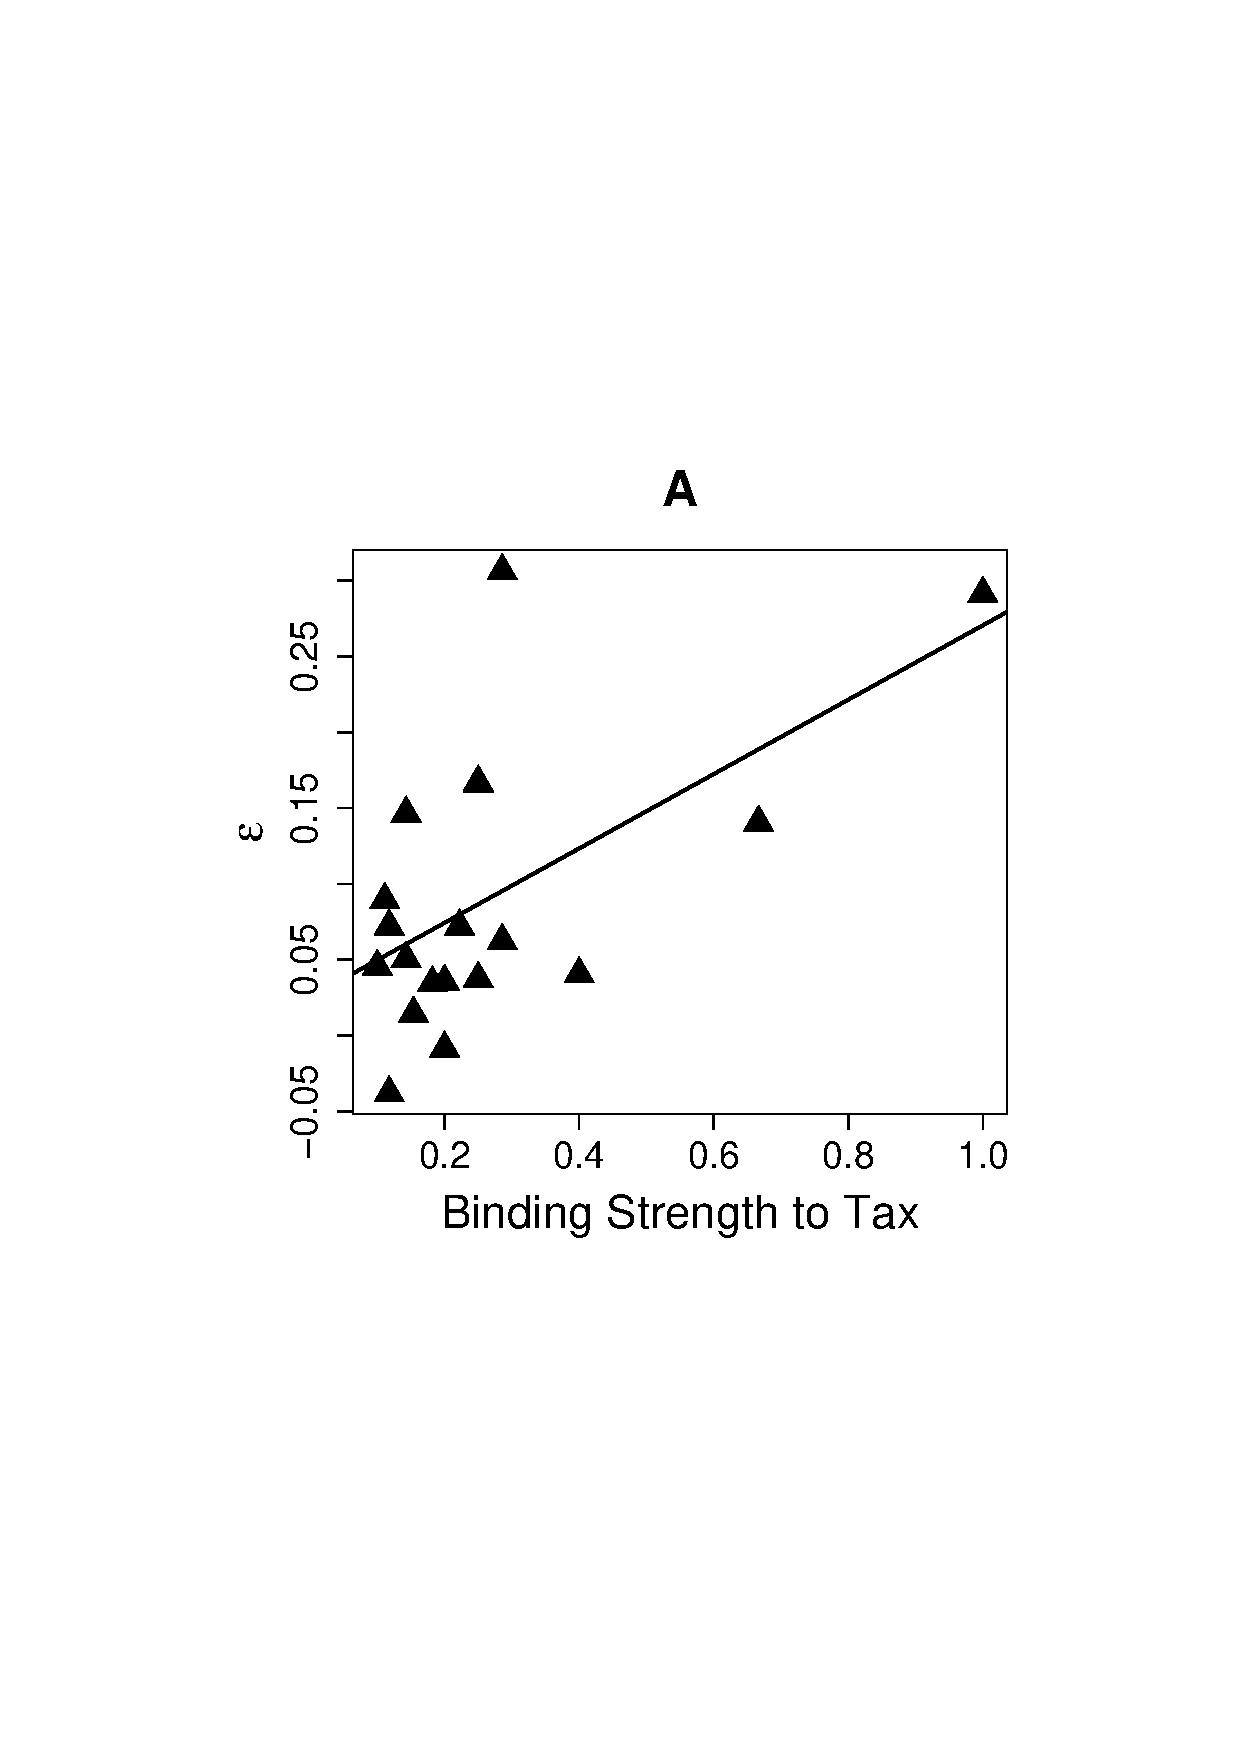
\includegraphics[width=10cm]{./Figures/chapter6/EpRank} \\
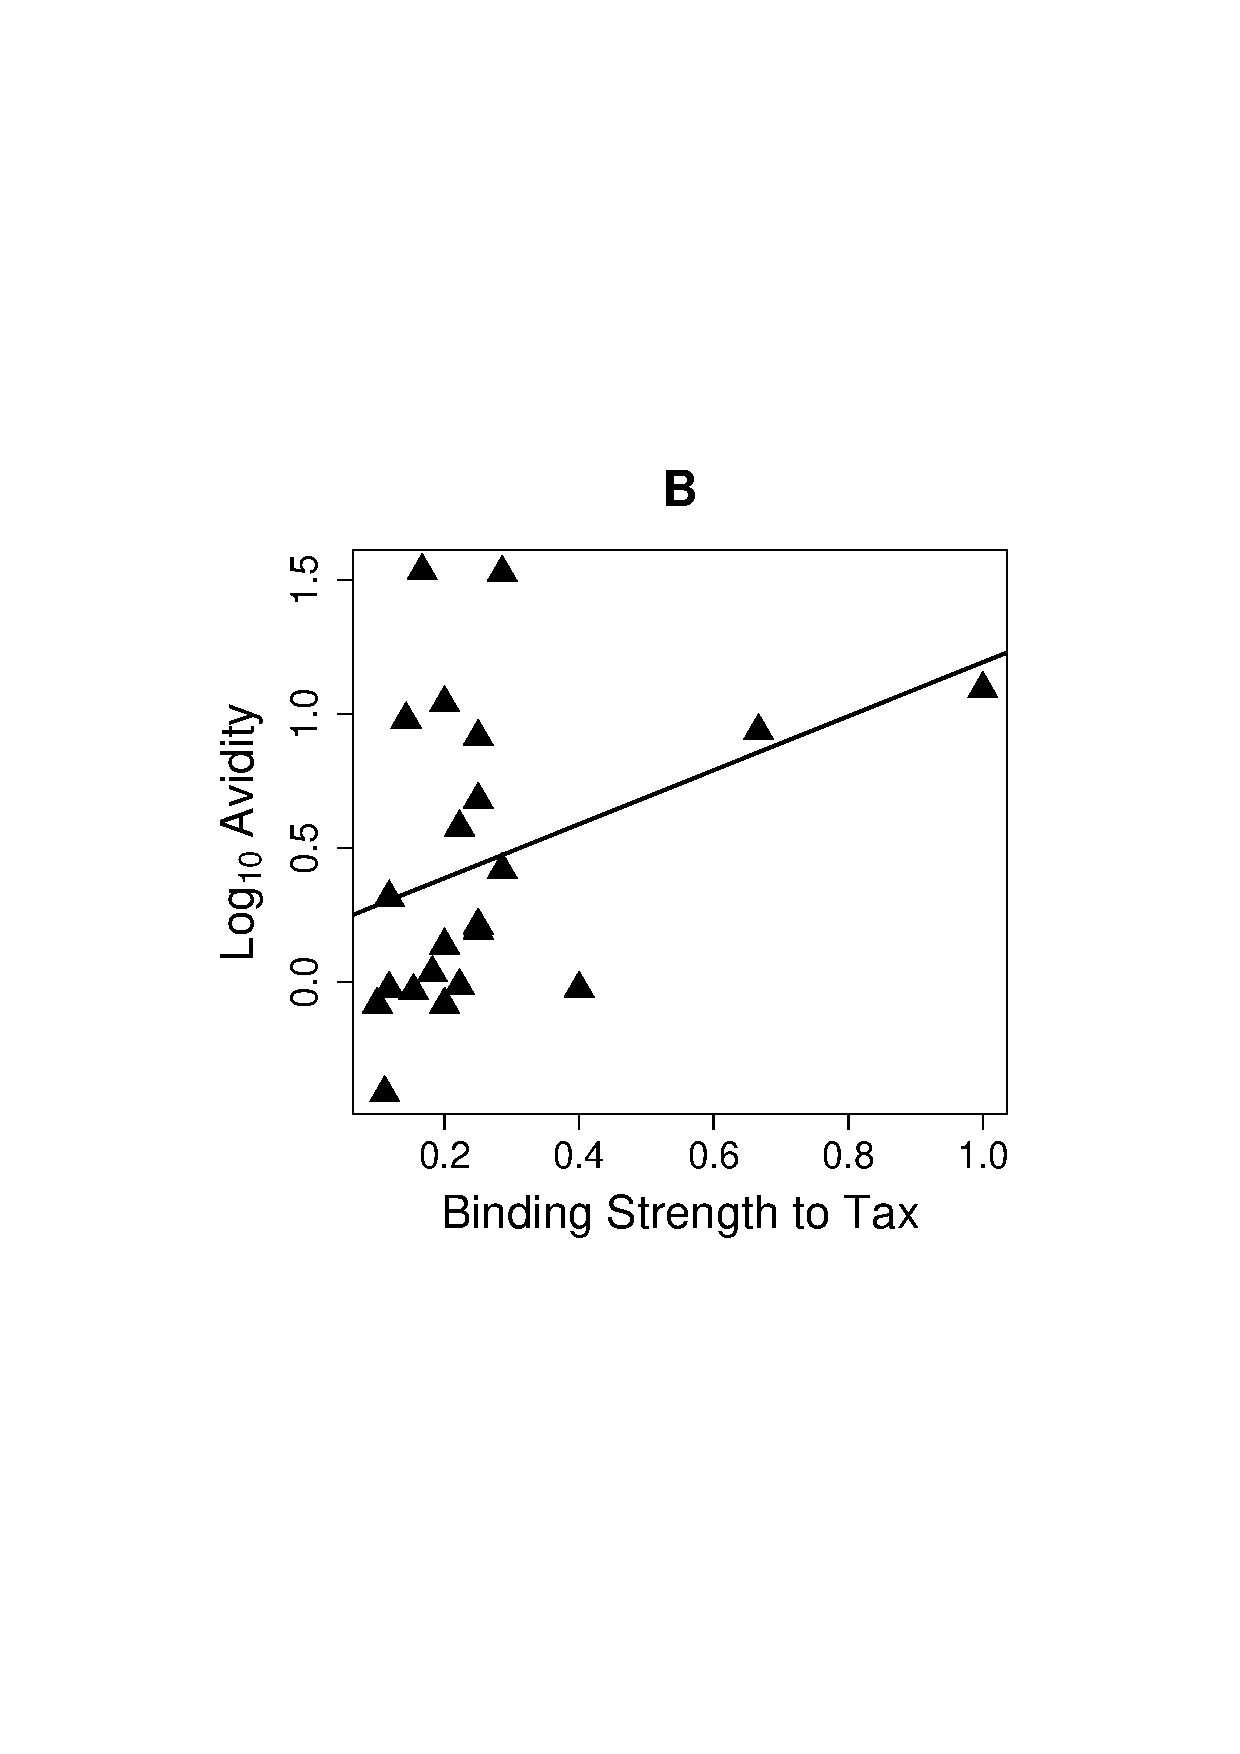
\includegraphics[width=10cm]{./Figures/chapter6/avidRank} \\
\caption[Measures of CD8$^+$ T cell efficacy and specificity of MHC class I]{A: The relationship between $\epsilon$ and the binding strength to Tax ($R^2 = 0.34$, $P = 0.008$). The binding strength to Tax is the reciprocal of the median rank value of the top binding Tax peptide to the individual's HLA class I repertoire (A, B and C alleles). B: The relationship between avidity ($10^6$ M$^{-1}$) and the binding strength to Tax ($R^2 = 0.14$, $P = 0.09$).}
\label{appendixc/figureRankComp}
\end{figure}

\clearpage

%%%%%%%%%%%%%%%%%%%%%%%%%%%%%%%%%%%%%%%%%%%%%%%%%%%%%%%%%%%%%%%%%%%%%%%%%%%%%%%%%%%%%%%%%%%%%%%%%%%%
%%%%%%%%%%%%%%%%%%%%%%%%%%%%%%%%%%%%%%%%%%%%%%%%%%%%%%%%%%%%%%%%%%%%%%%%%%%%%%%%%%%%%%%%%%%%%%%%%%%%

\begin{table}[htp]
\begin{center}
\begin{sideways}
{
\scriptsize
\begin{tabulary}{1.5\textwidth}{|c|c|c|c|c|c|c|c|c|c|c|c|c|}
\hline
& \multicolumn{2}{c|}{Pol} & \multicolumn{2}{c|}{Env} & \multicolumn{2}{c|}{Rof} & \multicolumn{2}{c|}{Tax} & \multicolumn{2}{c|}{P12} & \multicolumn{2}{c|}{Rex} \bigstrut \\
\hline
alleles & peptide & affinity & peptide & affinity & peptide & affinity & peptide & affinity & peptide & affinity & peptide & affinity \bigstrut \\
\hline
A0101 & HTDPRDQIY & 10 & SSSSTPLLY & 14 & PSDVSGLLL & 1153 & GSVVCMYLY & 703 & PSDVSGLLL & 1153 & QSTCLETVY & 917 \bigstrut[t] \\
A02 & ALLGEIQWV & 7.86207 & ALQTGITLV & 14.1921 & ILSGLLFLL & 16.1626 & YLYQLSPPI & 5.06404 & ILSGLLFLL & 16.1626 & IVTPYWPPV & 153.291\\
A0201 & YLYHYLRTL & 10 & VLYSPNVSV & 11 & ILSGLLFLL & 13 & LLFGYPVYV & 3 & ILSGLLFLL & 13 & SMDALSAQL & 72\\
A0203 & YLYHYLRTL & 3 & FLNTEPSQL & 2 & MLFRLLSPL & 2 & YLYQLSPPI & 3 & MLFRLLSPL & 2 & SLGDYVRPA & 4\\
A0206 & FQPYFAFTV & 2 & AQPVCSWTL & 8 & MLFRLLSPL & 15 & FLIPRLPSF & 4 & MLFRLLSPL & 15 & AQLYSSLSL & 7\\
A0301 & LLYKYFTDK & 7 & YLFPHWTKK & 9 & TMRFPARWR & 90 & FIFHKFQTK & 12 & TMRFPARWR & 90 & STCLETVYK & 665\\
A1101 & TTTVVFQSK & 7 & SSSSTPLLY & 24 & STMLFRLLS & 227 & QSSSFIFHK & 7 & PITMRFPAR & 2025 & STCLETVYK & 6\\
A2402 & KYKNTLYRL & 40 & KFLATLILF & 17 & LFLLFLPLF & 53 & SFHSLHLLF & 14 & LFLLFLPLF & 53 & PYWPPVQSI & 224\\
A26 & WTINHLNVL & 87.3461 & YTGAVSSPY & 73.1346 & PTPWQLPPF & 3523.25 & TTPGLIWTF & 173.75 & QILSGLLFL & 4815.65 & TGAPSLGDY & 7105.98\\
A2601 & WTINHLNVL & 105 & YTGAVSSPY & 83 & PTPWQLPPF & 4259 & TTPGLIWTF & 203 & QILSGLLFL & 5815 & TGAPSLGDY & 8542\\
A2602 & FTVPQQCNY & 2 & EVDKDISQL & 5 & AINPQLLHF & 8 & FLIPRLPSF & 6 & QILSGLLFL & 41 & TGAPSLGDY & 245\\
A3001 & RPWARTPPK & 8 & YLFPHWTKK & 11 & RRRPRRSQR & 102 & AMRKYSPFR & 4 & RFPARWRFL & 1347 & STCLETVYK & 58\\
A3101 & KVVYLHHVR & 7 & RQLRHLPSR & 6 & MPKTRRRPR & 17 & AMRKYSPFR & 3 & TMRFPARWR & 39 & MPKTRRRPR & 17\\
A3301 & ILRSCHACR & 23 & DLGLSQWAR & 7 & MPKTRRRPR & 50 & AMRKYSPFR & 119 & PITMRFPAR & 180 & MPKTRRRPR & 50\\
B0702 & APRNQPVPF & 8 & VPSSSSTPL & 5 & APSQPAAAF & 8 & SARLHRHAL & 7 & APSQPAAAF & 8 & RPAYIVTPY & 60\\
B1501 & KQFQPYFAF & 46 & YTGAVSSPY & 81 & SLQGLHLAF & 110 & GQHLPTLSF & 56 & FQILSGLLF & 61 & LSACTSTSF & 221\\
B3501 & FPQCTILQY & 14 & LPFNWTHCF & 6 & APSQPAAAF & 14 & IPPSFLQAM & 19 & APSQPAAAF & 14 & RPAYIVTPY & 8\\
B3901 & YHYLRTLAL & 6 & YHATYSLYL & 10 & LHFFFPSTM & 2596 & IQYSSFHSL & 147 & MRFPARWRF & 12998 & YKATGAPSL & 107\\
B40 & FEMQLAHIL & 44.9888 & WKFQHDVNF & 3789.06 & FQILSGLLF & 4594.8 & EELLYKISL & 39.8315 & FQILSGLLF & 4594.8 & AQLYSSLSL & 8671.56\\
B4001 & FEMQLAHIL & 11 & AQPVCSWTL & 1872 & FQILSGLLF & 3488 & EELLYKISL & 25 & FQILSGLLF & 3488 & AQLYSSLSL & 636\\
B4002 & FEMQLAHIL & 66 & REALQTGIT & 654 & FFFPSTMLF & 8666 & EELLYKISL & 49 & FQILSGLLF & 5279 & GEAPLSACT & 2863\\
B4402 & LEAGHIEPY & 593 & LENRVLTGW & 1253 & SQPAAAFLF & 8074 & EELLYKISL & 1037 & SQPAAAFLF & 8074 & MDALSAQLY & 12389\\
B5101 & LPMDNALSI & 13 & LPPFSLSPV & 11 & LPLLLSPSL & 26 & LPTTLFQPA & 42 & LPLLLSPSL & 26 & TPWPTSQGL & 445\\
B5401 & MPVFTLSPV & 4 & FPFSLLVDA & 2 & LPITMRFPA & 2 & LPTTLFQPA & 2 & LPITMRFPA & 2 & FPPPSPGPS & 59\\
B5801 & LTNCHKTRW & 32 & YSLYLFPHW & 13 & ITMRFPARW & 7 & RVIGSALQF & 32 & ITMRFPARW & 7 & LSACTSTSF & 74 \bigstrut[b] \\
\hline
\end{tabulary}
}
\end{sideways}
\end{center}
\caption[The top-ranking MHC class I - peptide binding affinities]{The top ranking MHC class I - peptide pairings for the alleles of the Kagoshima Cohort, according to the rank method (\sref{RankMeasure}).}	
\label{appendixc/table7}
\end{table}

\begin{table}[htp]
\begin{center}
\begin{sideways}
{
\scriptsize
\begin{tabulary}{1.5\textwidth}{|c|c|c|c|c|c|c|c|c|c|c|c|c|}
\hline
& \multicolumn{2}{c|}{HBZ} & \multicolumn{2}{c|}{Gag} & \multicolumn{2}{c|}{Pro} & \multicolumn{2}{c|}{Tof} & \multicolumn{2}{c|}{P13} & \multicolumn{2}{c|}{P21} \bigstrut \\
\hline
alleles & peptide & affinity & peptide & affinity & peptide & affinity & peptide & affinity & peptide & affinity & peptide & affinity \bigstrut \\
\hline
A0101 & MQELGIDGY & 6029 & WLNFLQAAY & 2442 & LQQCQGVLY & 6429 & FSSSFLFKY & 32 & YRLSSTVPY & 20283 & LSACTSTSF & 6727 \bigstrut[t] \\
A02 & AVLDGLLSL & 19.9557 & FMQTIRLAV & 8.75862 & ALFSSNTPL & 18.7783 & LIISPLPRV & 42.4385 & LIISPLPRV & 42.4385 & AQLYSSLSL & 352.256\\
A0201 & AVLDGLLSL & 31 & FMQTIRLAV & 7 & ALFSSNTPL & 11 & LTMLIISPL & 73 & LIISPLPRV & 63 & EMDTWNPPL & 86\\
A0203 & ELVDGLLSL & 19 & FMQTIRLAV & 5 & RLPFRTTPI & 3 & LTMLIISPL & 21 & RLVPHLWGT & 11 & ALSAQLYSS & 61\\
A0206 & AVLDGLLSL & 3 & WQMKDLQAI & 2 & IQAPAVLGL & 29 & RLVPHLWGT & 2 & RLVPHLWGT & 2 & AQLYSSLSL & 7\\
A0301 & KAKQHSARK & 145 & SLLASLLPK & 18 & GITQYSQLK & 77 & SLSFNSSSK & 19 & SSFRIPSLR & 87 & PTFHPPSSR & 1782\\
A1101 & KAADVARRK & 55 & SSYDFHQLK & 4 & GITQYSQLK & 34 & SSFSRSFFR & 3 & SSFRIPSLR & 14 & PTFHPPSSR & 482\\
A2402 & YWQGRLEAM & 4434 & GYPGRVNEI & 40 & PFRTTPIVL & 2930 & SFSRSFFRF & 12 & VWTESSFRI & 35 & QSLIQPPTF & 2171\\
A26 & ELVDGLLSL & 52.8654 & ETPARICPI & 182.25 & DTKNNWAII & 190.25 & LVPHLWGTM & 1229.29 & LVPHLWGTM & 1229.29 & CTPSGEAPL & 9512.65\\
A2601 & ELVDGLLSL & 61 & ETPARICPI & 216 & DTKNNWAII & 215 & FSSSFLFKY & 2530 & LVPHLWGTM & 1478 & CTPSGEAPL & 11277\\
A2602 & ELVDGLLSL & 14 & HTNSPLGDM & 13 & MTVLPIALF & 4 & LVPHLWGTM & 41 & LVPHLWGTM & 41 & EMDTWNPPL & 908\\
A3001 & KAKQHSARK & 6 & KVLVVQPKK & 5 & LFSSNTPLK & 57 & AFSSSFLFK & 43 & MLIISPLPR & 683 & RSLPRQSLI & 1219\\
A3101 & RQRRAEEKR & 43 & WSRDCTQPR & 61 & NTWSGRPWR & 16 & SSFSRSFFR & 2 & RVWRLCTRR & 4 & PTFHPPSSR & 427\\
A3301 & EVESLEAER & 23 & EPYHAFVER & 89 & NTWSGRPWR & 11 & SSFSRSFFR & 7 & HLGPHRWTR & 12 & PTFHPPSSR & 1332\\
B0702 & LPVSCPEDL & 171 & RPPPGPCPL & 9 & LPVLIRLPF & 7 & GPRRSRPRL & 9 & VPYPSTPLL & 33 & PPSPPREPL & 50\\
B1501 & MQELGIDGY & 230 & YQQLWLAAF & 53 & LQQCQGVLY & 147 & FLLATSAAF & 65 & YRLSSTVPY & 1909 & LSACTSTSF & 221\\
B3501 & MQELGIDGY & 492 & DPILRSLAY & 10 & LPVLIRLPF & 9 & VPHLWGTMF & 12 & VPHLWGTMF & 12 & MDALSAQLY & 401\\
B3901 & DKEEEKAVL & 1540 & FVERLNIAL & 330 & SHPKTIEAL & 219 & RRAFSSSFL & 2708 & PHRWTRYRL & 5300 & EMDTWNPPL & 507\\
B40 & EEKQIAEYL & 203.775 & LEEPYHAFV & 434.978 & PEAKRPPVI & 4188.22 & RAFSSSFLF & 13314 & YRLSSTVPY & 35018.8 & AQLYSSLSL & 8671.56\\
B4001 & VEELVDGLL & 260 & EEDALLLDL & 112 & GQTQDHFKL & 406 & RAFSSSFLF & 17075 & YRLSSTVPY & 36290 & AQLYSSLSL & 636\\
B4002 & EEKQIAEYL & 148 & REYQQLWLA & 248 & PEAKRPPVI & 2102 & RAFSSSFLF & 10989 & VPHLWGTMF & 21041 & GEAPLSACT & 2863\\
B4402 & EEEKQIAEY & 295 & AETRGITGY & 231 & LQQCQGVLY & 16483 & SFSRSFFRF & 8791 & SDHLGPHRW & 7122 & MDALSAQLY & 12389\\
B5101 & LPVSCPEDL & 246 & LPKGYPGRV & 185 & LPFRTTPIV & 21 & VPYPSTPLL & 204 & VPYPSTPLL & 204 & LPRQSLIQP & 375\\
B5401 & LPVSCPEDL & 2433 & LPVMHPHGA & 7 & LPVIPLDPA & 2 & RPTGHLSRA & 1054 & RPTGHLSRA & 1054 & FPPPSPGPS & 59\\
B5801 & DLMGEVNYW & 1488 & QAAPGSPQF & 70 & NASRPCNTW & 140 & RAFSSSFLF & 9 & IISPLPRVW & 31 & LSACTSTSF & 74 \bigstrut[b] \\
\hline
\end{tabulary}
}
\end{sideways}
\end{center}
\contcaption{Continued}
\end{table}

%%%%%%%%%%%%%%%%%%%%%%%%%%%%%%%%%%%%%%%%%%%%%%%%%%%%%%%%%%%%%%%%%%%%%%%%%%%%%%%%%%%%%%%%%%%%%%%%%%%%
%%%%%%%%%%%%%%%%%%%%%%%%%%%%%%%%%%%%%%%%%%%%%%%%%%%%%%%%%%%%%%%%%%%%%%%%%%%%%%%%%%%%%%%%%%%%%%%%%%%%

\begin{table}[htp]
\begin{center}
\begin{sideways}
\begin{tabulary}{1.5\textwidth}{|c|c|c|c|c|c|c|c|c|c|}
\hline
Peptide & A0201 & B0702 & A2402 & B3501 & Peptide & A0201 & B0702 & A2402 & B3501 \bigstrut \\
\hline
AAGAALIPV & YES &  &  &  & GLLSLEEEL & YES &  &  &  \bigstrut[t] \\
AAHHWLNFL & YES & YES &  & YES & GYPGRVNEI &  &  & YES &  \\
AASGLFRCL &  & YES &  & YES & GYTRQLEGE &  &  & YES &  \\
ALLGEIQWV & YES &  &  &  & HPGQLGAFL &  & YES &  & YES \\
APLPHTSQC &  & YES &  &  & HQLKKFLKI & YES &  & YES &  \\
APPPPSSPT &  & YES &  &  & IALETPARI & YES &  & YES &  \\
ASGLFRCLP & YES & YES & YES & YES & ICPINYSLL &  &  & YES &  \\
AVLDGLLSL & YES & YES & YES & YES & IFSRSASPI &  &  & YES &  \\
AWQNGLLPF &  &  & YES &  & ILIQTQAQI & YES &  &  &  \\
CPINYSLLA &  &  &  & YES & ILPEDCLPT & YES &  &  &  \\
CPLCQDPTH &  &  &  & YES & IPPSFLQAM &  & YES &  & YES \\
DLMGEVNYW &  &  & YES &  & IPRLPSFPT &  & YES &  &  \\
DPILRSLAY &  &  &  & YES & IPRPPRGLA &  & YES &  &  \\
DPISRLNAL &  & YES &  & YES & IQYSSFHSL & YES & YES & YES &  \\
EEEKQIAEY &  &  &  & YES & IWQGDITHF &  &  & YES &  \\
EKAVLDGLL &  &  & YES &  & KALMPVFTL & YES & YES & YES & YES \\
ELVDGLLSL & YES &  &  & YES & KARRRRRAE &  & YES &  &  \\
EPEEDALLL &  &  &  & YES & KISLTTGAL & YES & YES &  &  \\
EPEPEEDAL &  &  &  & YES & KLLQEKEDL & YES &  &  &  \\
EPGPSSYDF &  &  &  & YES & KQIAEYLKR &  &  & YES &  \\
EYLKRKEEE &  &  & YES &  & KYKNTLYRL &  &  & YES &  \\
EYQQLWLAA &  &  & YES &  & KYLYHYLRT &  &  & YES &  \\
EYTNIPISL &  &  & YES &  & KYTLQSYGL &  &  & YES &  \\
FMQTIRLAV & YES &  &  &  & LAAHHWLNF &  & YES & YES & YES \\
FPGFGQSLL &  & YES &  & YES & LASLLPKGY &  &  &  & YES \\
FPQCTILQY &  &  &  & YES & LEAERRKLL &  & YES &  &  \\
FPTQRTSKT &  &  &  & YES & LLFGYPVYV & YES &  &  &  \\
FVERLNIAL & YES & YES &  & YES & LLITPVLQL & YES &  &  &  \\
GFGQSLLFG & YES & YES & YES & YES & LLLDLPADI & YES &  &  &  \\
GIDGYTRQL & YES &  &  &  & LLQEKEDLM & YES &  &  & YES \bigstrut[b] \\
\hline
\end{tabulary}
\end{sideways}
\end{center}
\caption[The REVEAL\superscript{TM} binding assay peptides]{The HTLV-I peptides that were selected for the REVEAL\superscript{TM} MHC-peptide binding assay, for each allele. These were compared against the predicted binding affinities of Metaserver and Epipred.}
\label{appendixc/table1}
\end{table}


\begin{table}[htp]
\begin{center}
\begin{sideways}
\begin{tabulary}{1.5\textwidth}{|c|c|c|c|c|c|c|c|c|c|}
\hline
Peptide & A0201 & B0702 & A2402 & B3501 & Peptide & A0201 & B0702 & A2402 & B3501 \bigstrut \\
\hline
LLQYLCSSL & YES &  &  &  & QPARAPVTL &  & YES &  & YES \bigstrut[t] \\
LLYKISLTT & YES &  &  &  & QPIPETRSL &  & YES &  &  \\
LMGEVNYWQ & YES &  &  &  & QPRPPPGPC &  & YES &  &  \\
LPEDCLPTT &  &  &  & YES & QYLCSSLVA &  &  & YES &  \\
LPFHSTLTT &  & YES &  & YES & RAEKKAADV &  & YES &  &  \\
LPGLNSRQW &  & YES &  &  & RDRQRRAEE &  & YES &  &  \\
LPTTLFQPA &  &  &  & YES & RGRLRRGPP &  & YES &  &  \\
LPVMHPHGA &  & YES &  &  & RICPINYSL & YES & YES & YES &  \\
LPVSCPEDL &  & YES &  & YES & RPAPPPPSS &  & YES &  &  \\
LQYLCSSLV & YES &  &  &  & RPPPGPCPL &  & YES &  &  \\
LSPPITWPL & YES &  & YES & YES & RPPRGLAAH &  & YES &  & YES \\
LTPPITHTT & YES &  &  & YES & RRRAEKKAA &  & YES &  &  \\
LVEELVDGL & YES &  &  & YES & RVIGSALQF &  & YES & YES & YES \\
LVLQSSSFI & YES & YES &  &  & RVNEILHIL & YES & YES &  & YES \\
LWLAAFAAL &  &  & YES &  & SAQWIPWRL & YES & YES & YES & YES \\
MPVFTLSPV &  & YES &  & YES & SARLHRHAL &  & YES &  &  \\
MQELGIDGY &  &  &  & YES & SFHSLHLLF &  &  & YES &  \\
NFLQAAYRL &  &  & YES & YES & SFLLSHGLI &  &  & YES &  \\
NYSLLASLL &  &  & YES &  & SLVQLRQAL & YES & YES &  & YES \\
PPNHRPWQM &  & YES &  &  & STLTTPGLI & YES &  & YES &  \\
PYHAFVERL &  &  & YES &  & SWASILQGL &  &  & YES &  \\
PYKRIEELL &  &  & YES &  & SYGLLCQTI &  &  & YES &  \\
PYNPTSSGL &  &  & YES &  & TFLKTAAPL &  & YES & YES &  \\
QAAPGSPQF &  &  &  & YES & TLGQHLPTL & YES &  &  &  \\
QAMRKYSPF &  & YES & YES & YES & TLSFPDPGL & YES &  &  &  \\
QLDSLISEA & YES &  &  &  & TLTAWQNGL & YES &  &  &  \\
QLEGEVESL & YES &  &  &  & TLYRLHVWV & YES &  &  &  \\
QLGAFLTNV & YES &  &  &  & TPKDKTKVL &  & YES &  &  \\
QLLASAVLL & YES &  &  &  & TPNIPPSFL &  & YES &  &  \\
QLWLAAFAA & YES &  &  &  & TTPGLIWTF &  &  & YES & \bigstrut[b] \\
\hline
\end{tabulary}
\end{sideways}
\end{center}
\contcaption{Continued}
\end{table}


\begin{table}[htp]
\begin{center}
\begin{sideways}
\begin{tabulary}{1.5\textwidth}{|c|c|c|c|c|}
\hline
Peptide & A0201 & B0702 & A2402 & B3501 \bigstrut \\
\hline
TTPNIPPSF &  &  & YES &  \bigstrut[t] \\
TWPLLPHVI &  &  & YES &  \\
VFTLSPVII &  &  & YES &  \\
VLQSSSFIF &  &  & YES &  \\
VPIRSRWAL &  & YES &  &  \\
VPYKRIEEL &  & YES &  &  \\
VSCPEDLLV &  &  & YES &  \\
WALPELQAL &  &  &  & YES \\
WPLLPHVIF &  &  &  & YES \\
WQGRLEAMW &  &  & YES &  \\
WQMKDLQAI & YES &  & YES &  \\
WTFTDGTPM &  &  &  & YES \\
WTINHLNVL &  &  &  & YES \\
YILWDKQIL & YES &  &  & YES \\
YISQDFLNM & YES &  &  & YES \\
YLCSSLVAS & YES &  &  &  \\
YLYQLSPPI & YES &  &  &  \\
YPGRVNEIL &  & YES &  & YES \\
YWQGRLEAM &  &  & YES & YES \bigstrut[b] \\
\hline
\end{tabulary}
\end{sideways}
\end{center}
\contcaption{Continued}
\end{table}

%%%%%%%%%%%%%%%%%%%%%%%%%%%%%%%%%%%%%%%%%%%%%%%%%%%%%%%%%%%%%%%%%%%%%%%%%%%%%%%%%%%%%%%%%%%%%%%%%%%%
%%%%%%%%%%%%%%%%%%%%%%%%%%%%%%%%%%%%%%%%%%%%%%%%%%%%%%%%%%%%%%%%%%%%%%%%%%%%%%%%%%%%%%%%%%%%%%%%%%%%

\begin{table}[htp]
\begin{center}
\begin{tabulary}{\textwidth}{|L|}
\hline
Gag \bigstrut[t] \\
MGQIFSRSASPIPRPPRGLAAHHWLNFLQAAYRLEPGPSSYDFHQLKKFL \bigstrut[t] \\
KIALETPARICPINYSLLASLLPKGYPGRVNEILHILIQTQAQIPSRPAP \\
PPPSSPTHDPPDSDPQIPPPYVEPTAPQVLPVMHPHGAPPNHRPWQMKDL \\
QAIKQEVSQAAPGSPQFMQTIRLAVQQFDPTAKDLQDLLQYLCSSLVASL \\
HHQQLDSLISEAETRGITGYNPLAGPLRVQANNPQQQGLRREYQQLWLAA \\
FAALPGSAKDPSWASILQGLEEPYHAFVERLNIALDNGLPEGTPKDPILR \\
SLAYSNANKECQKLLQARGHTNSPLGDMLRACQTWTPKDKTKVLVVQPKK \\
PPPNQPCFRCGKAGHWSRDCTQPRPPPGPCPLCQDPTHWKRDCPRLKPTI \\
PEPEPEEDALLLDLPADIPHPKNFIGGEV \bigstrut[b] \\
\hline
Env \bigstrut[t] \\
MGKFLATLILFFQFCPLIFGDYSPSCCTLTIGVSSYHSKPCNPAQPVCSW \bigstrut[t] \\
TLDLLALSADQALQPPCPNLVSYSSYHATYSLYLFPHWTKKPNRNGGGYY \\
SASYSDPCSLKCPYLGCQSWTCPYTGAVSSPYWKFQHDVNFTQEVSRLNI \\
NLHFSKCGFPFSLLVDAPGYDPIWFLNTEPSQLPPTAPPLLPHSNLDHIL \\
EPSIPWKSKLLTLVQLTLQSTNYTCIVCIDRASLSTWHVLYSPNVSVPSS \\
SSTPLLYPSLALPAPHLTLPFNWTHCFDPQIQAIVSSPCHNSLILPPFSL \\
SPVPTLGSRSRRAVPVAVWLVSALAMGAGVAGGITGSMSLASGKSLLHEV \\
DKDISQLTQAIVKNHKNLLKIAQYAAQNRRGLDLLFWEQGGLCKALQEQC \\
RFPNITNSHVPILQERPPLENRVLTGWGLNWDLGLSQWAREALQTGITLV \\
ALLLLVILAGPCILRQLRHLPSRVRYPHYSLIKPESSL \bigstrut[b] \\
\hline
Pro \bigstrut[t] \\
HPTPKKLHRGGGLTSPPTLQQVLPNQDPASILPVIPLDPARRPVIKAQVD \bigstrut[t] \\
TQTSHPKTIEALLDTGADMTVLPIALFSSNTPLKNTSVLGAGGQTQDHFK \\
LTSLPVLIRLPFRTTPIVLTSCLVDTKNNWAIIGRDALQQCQGVLYLPEA \\
KRPPVILPIQAPAVLGLEHLPRPPEISQFPLNQNASRPCNTWSGRPWRQA \\
ISNPTPGQGITQYSQLKRPMEPGDSSTTCGPLTL \bigstrut[b] \\
\hline
Pol \bigstrut[t] \\
GKKAACNLANTGASRPWARTPPKAPRNQPVPFKPERLQALQHLVRKALEA \bigstrut[t] \\
GHIEPYTGPGNNPVFPVKKANGTWRFIHDLRATNSLTIDLSSSSPGPPDL \\
SSLPTTLAHLQTIDLRDAFFQIPLPKQFQPYFAFTVPQQCNYGPGTRYAW \\
KVLPQGFKNSPTLFEMQLAHILQPIRQAFPQCTILQYMDDILLASPSHED \\
LLLLSEATMASLISHGLPVSENKTQQTPGTIKFLGQIISPNHLTYDAVPT \\
VPIRSRWALPELQALLGEIQWVSKGTPTLRQPLHSLYCALQRHTDPRDQI \\
YLNPSQVQSLVQLRQALSQNCRSRLVQTLPLLGAIMLTLTGTTTVVFQSK \\
EQWPLVWLHAPLPHTSQCPWGQLLASAVLLLDKYTLQSYGLLCQTIHHNI \\
STQTFNQFIQTSDHPSVPILLHHSHRFKNLGAQTGELWNTFLKTAAPLAP \\
VKALMPVFTLSPVIINTAPCLFSDGSTSRAAYILWDKQILSQRSFPLPPP \\
HKSAQRAELLGLLHGLSSARSWRCLNIFLDSKYLYHYLRTLALGTFQGRS \\
SQAPFQALLPRLLSRKVVYLHHVRSHTNLPDPISRLNALTDALLITPVLQ \\
LSPAELHSFTHCGQTALTLQGATTTEASNILRSCHACRGGNPQHQMPRGH \\
IRRGLLPNHIWQGDITHFKYKNTLYRLHVWVDTFSGAISATQKRKETSSE \\
AISSLLQAIAHLGKPSYINTDNGPAYISQDFLNMCTSLAIRHTTHVPYNP \\
TSSGLVERSNGILKTLLYKYFTDKPDLPMDNALSIALWTINHLNVLTNCH \\
KTRWQLHHSPRLQPIPETRSLSNKQTHWYYFKLPGLNSRQWKGPQEALQE \\
AAGAALIPVSASSAQWIPWRLLKRAACPRPVGGPADPKEKDLQHHG \bigstrut[b] \\
\hline
\end{tabulary}
\end{center}
\caption[The HTLV-I proteome]{The HTLV-I proteome. This reference strain is from \citep{Seiki1983}, with the exception of HBZ, which was identified more recently and described in \citep{Satou2006}.}\label{appendixc/table2}
\end{table}

\begin{table}[htp]
\begin{center}
\begin{tabulary}{\textwidth}{|L|}
\hline
Rof \bigstrut[t] \\
MPKTRRRPRRSQRKRPPTPWQLPPFSLQGLHLAFQLSSIAINPQLLHFFF \bigstrut[t] \\
PSTMLFRLLSPLSPLALTALLLFLLPPSDVSGLLLRPPPAPCLLLFLPFQ \\
ILSGLLFLLFLPLFFSLPLLLSPSLPITMRFPARWRFLPWRAPSQPAAAF \\
LF \bigstrut[b] \\
\hline
P12 \bigstrut[t] \\
MLFRLLSPLSPLALTALLLFLLPPSDVSGLLLRPPPAPCLLLFLPFQILS \bigstrut[t] \\
GLLFLLFLPLFFSLPLLLSPSLPITMRFPARWRFLPWRAPSQPAAAFLF \bigstrut[b] \\
\hline
Tof \bigstrut[t] \\
MALCCFAFSAPCLHLRSRRSCSSCFLLATSAAFFSARLLRRAFSSSFLFK \bigstrut[t] \\
YSAVCFSSSFSRSFFRFLFSSARRCRSRCVSPRGGAFSPGGPRRSRPRLS \\
SSKDSKPSSTASSSSLSFNSSSKDNSPSTNSSTSRSSGHDTGKHRNSPAD \\
TKLTMLIISPLPRVWTESSFRIPSLRVWRLCTRRLVPHLWGTMFGPPTSS \\
RPTGHLSRASDHLGPHRWTRYRLSSTVPYPSTPLLPHPENL \bigstrut[b] \\
\hline 
P13 \bigstrut[t] \\
MLIISPLPRVWTESSFRIPSLRVWRLCTRRLVPHLWGTMFGPPTSSRPTG \bigstrut[t] \\
HLSRASDHLGPHRWTRYRLSSTVPYPSTPLLPHPENL \bigstrut[b] \\
\hline
Rex \bigstrut[t] \\
MPKTRRRPRRSQRKRPPTPWPTSQGLDRVFFSDTQSTCLETVYKATGAPS \bigstrut[t] \\
LGDYVRPAYIVTPYWPPVQSIRSPGTPSMDALSAQLYSSLSLDSPPSPPR \\
EPLRPSRSLPRQSLIQPPTFHPPSSRPCANTPPSEMDTWNPPLGSTSQPC \\
LFQTPDSGPKTCTPSGEAPLSACTSTSFPPPSPGPSCPT \bigstrut[b] \\
\hline
P21 \bigstrut[t] \\
MDALSAQLYSSLSLDSPPSPPREPLRPSRSLPRQSLIQPPTFHPPSSRPC \bigstrut[t] \\
ANTPPSEMDTWNPPLGSTSQPCLFQTPDSGPKTCTPSGEAPLSACTSTSF \\
PPPSPGPSCPT \bigstrut[b] \\
\hline
Tax \bigstrut[t] \\
MAHFPGFGQSLLFGYPVYVFGDCVQGDWCPISGGLCSARLHRHALLATCP \bigstrut[t] \\
EHQITWDPIDGRVIGSALQFLIPRLPSFPTQRTSKTLKVLTPPITHTTPN \\
IPPSFLQAMRKYSPFRNGYMEPTLGQHLPTLSFPDPGLRPQNLYTLWGGS \\
VVCMYLYQLSPPITWPLLPHVIFCHPGQLGAFLTNVPYKRIEELLYKISL \\
TTGALIILPEDCLPTTLFQPARAPVTLTAWQNGLLPFHSTLTTPGLIWTF \\
TDGTPMISGPCPKDGQPSLVLQSSSFIFHKFQTKAYHPSFLLSHGLIQYS \\
SFHSLHLLFEEYTNIPISLLFNEKEADDNDHEPQISPGGLEPPSEKHFRE \\
TEV \bigstrut[b] \\
\hline
HBZ \bigstrut[t] \\
MAASGLFRCLPVSCPEDLLVEELVDGLLSLEEELKDKEEEKAVLDGLLSL \bigstrut[t] \\
EEESRGRLRRGPPGEKAPPRGETHRDRQRRAEEKRKRKKEREKEEEKQIA \\
EYLKRKEEEKARRRRRAEKKAADVARRKQEEQERRERKWRQGAEKAKQHS \\
ARKEKMQELGIDGYTRQLEGEVESLEAERRKLLQEKEDLMGEVNYWQGRL \\
EAMWLQ \bigstrut[b] \\
\hline
\end{tabulary}
\end{center}
\contcaption{Continued}
\end{table}

%%%%%%%%%%%%%%%%%%%%%%%%%%%%%%%%%%%%%%%%%%%%%%%%%%%%%%%%%%%%%%%%%%%%%%%%%%%%%%%%%%%%%%%%%%%%%%%%%%%%
%%%%%%%%%%%%%%%%%%%%%%%%%%%%%%%%%%%%%%%%%%%%%%%%%%%%%%%%%%%%%%%%%%%%%%%%%%%%%%%%%%%%%%%%%%%%%%%%%%%%